\section{Zadání}

Pomocí numerických experimentů ověřte základní statistické vlastnosti odhadů klasického a klasického normálního modelu uvedených v Gauss-Markovově větě.
Zaměřte se například na ověření:

\begin{itemize}
    \item nestrannosti odhadů parametrů \( \beta_0, \beta_1 \),\ldots;
    \item nestrannosti odhadu \( \sigma^2 \);
    \item normality odhadů parametrů pro klasický normální regresní model.
\end{itemize}

\section{Teorie}

Polynomiální regrese prvního stupně, známa též jako lineární regrese je jednou ze základních matematických metod.
Výstupem metody je proložení souboru vstupních dat (bodů) v n-dimenzionálnním prostoru přímkou.
Díky své jednoduchosti a rychlosti výpočtu nachází tato metoda uplatnění v mnoha oborech, např. strojovém učení.

Přímkový regresní model je vyjádřen následujícím vztahem.

\begin{equation}
    Y_i = \beta_0 + \beta_1 X_i + \epsilon_i; \: i = 1,2,\ldots,n
\end{equation}

Odhad lineárního modelu je možné provést několika různýmy způsoby, nejčastěji však metodou nejmenších čtverců (\textit{Mean Squared Error}).

\begin{equation}
    \widehat{MSE}(\beta_0, \beta_1) \equiv \frac{1}{n}\sum_{i=1}^{n}{(y_i - (\beta_0 + \beta_1 x_i))^2}
\end{equation}

Při odhadu parametrů provádíme minimalizaci ztrátové funkce.

\begin{align}
    {minimize} \frac{1}{n} \sum_{i = 1}^{n} ({pred}_i - y_i)^2 \\
    J = \frac{1}{n} \sum_{i = 1}^{n} ({pred}_i - y_i)^2
\end{align}

Dle teorie přednášek (konkrétně přednáška 2, část 2) předpokládáme, že odhad parametrů metodou nejmenších čtverců je nejlepší nestranný lineární odhad (\textit{Best Linear Unbiased Estimator}).
Nestrannost odhadů parametrů znamená, že očekávaná hodnota (tj. střední hodnota - \textit{expected}) odhadů je rovna hodnotě parametrů samotných.

\begin{equation}
    E(b_i) = \beta_i
\end{equation}

Zajímavý pohled na MNČ jako na funkci lineární kombinace parametrů \( \theta \).

\begin{align}
    \theta = a_0 \beta_0 + a_1 \beta_1 \\
    \hat{\theta} = a_0 b_0 + a_1 b_1
\end{align}

\( \hat{\theta} \) je odhadem regresní přímky, \( a_0 = 1, \: a_1 = x\) jsou libovolná reálná čísla.
Potom lze uvažovat MSE jako rozptyl veličiny \( \hat{\theta} - \theta \).

\begin{equation}
    {MSE}(\hat{\theta}) \triangleq \mathbb{E} \left[( \hat{\theta} - \theta)^{2}\right]
\end{equation}

Střední kvadratická chyba je tudííž vždy nezáporná a nulová pouze v případě, kdy je odhad bezchybný.
Vlastností takto definované střední kvadratické chyby je, že se dá rozložit na součet systematické chyby (vychýlení) a rozptylu odhadu (náhodná nepřesnost odhadu).

\begin{equation}
    {MSE}(\hat{\theta}) = {Bias}(\hat{\theta})^{2} + {Var}(\hat{\theta})
\end{equation}

Jestliže budeme požadovat konstrukci intervalových odhadů a testů hypotéz, tak bude třeba přidat předpoklad normality dat pro náhodný vektor.
V tom případě má náhodná veličina \( \hat{\theta} \) normální rozdělení pravděpodobnosti s následující střední hodnotou a rozptylem.

\begin{align}
    E(\hat{\theta}) = a_0 \beta_0 + a_1 \beta_1 \\
    var(\hat{\theta}) = \sigma^2 v^2(a_1, a_2)
\end{align}

\section{Vypracování}

V rámci vypracování počítáme dolní a horní odhady pro intervaly spolehlivosti.
Výsledky jsou zaznamenány na grafu~\ref{fig:lr1}.
Pouhýh několik výsledků z evšech provedených simulací se nachází mimo očekávané hodnoty.

\begin{figure}[htb]
    \centering
    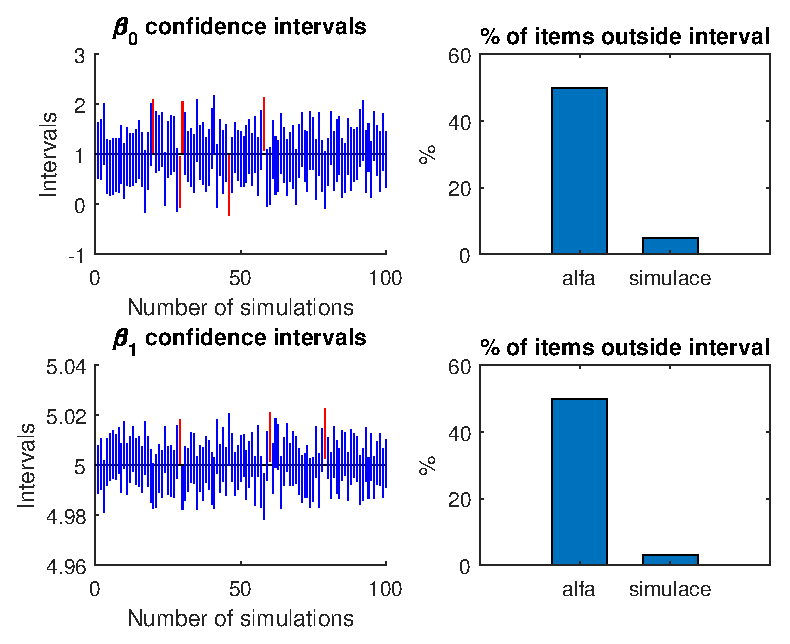
\includegraphics[width=0.55\textwidth]{graphs/fig1.eps}
    \caption{Vývoj dolních a horních odhadů parametrů \( \beta_i \)}
    \label{fig:lr1}
\end{figure}
\FloatBarrier

Na následujícím grafu lze zhodnotit, že četnosti odhadů parametrů \( \beta_i \) mají Gaussovo rozložení.

\begin{figure}[htb]
    \centering
    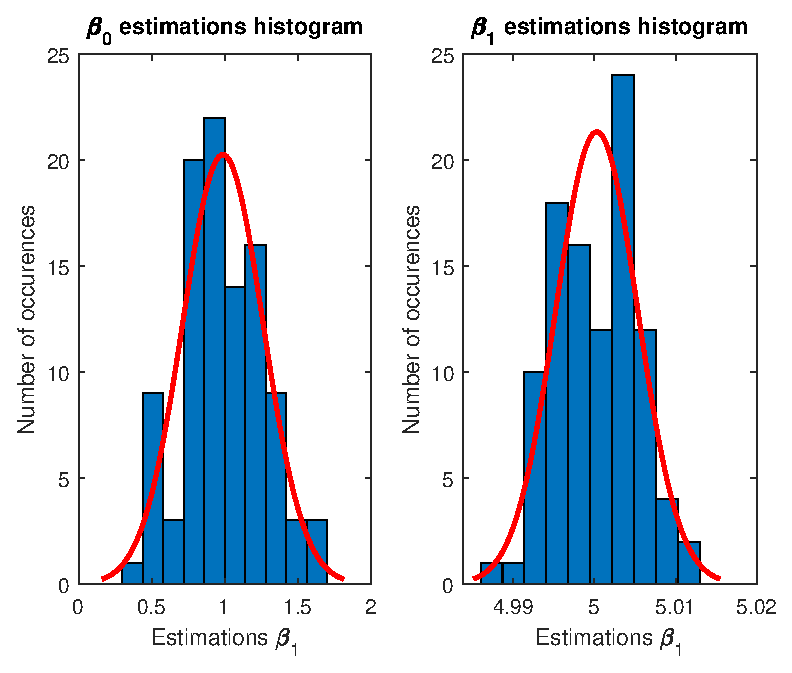
\includegraphics[width=0.55\textwidth]{graphs/fig2.eps}
    \caption{Četnosti hodnot \( \beta_0, \: \beta_1 \) napříč simulacemi.}
    \label{fig:lr2}
\end{figure}
\FloatBarrier

Na posledním grafu je znázorněna konvergence odhadů k teoretickým hodnotám pro zvyšující se počet dat.

\begin{figure}[htb]
    \centering
    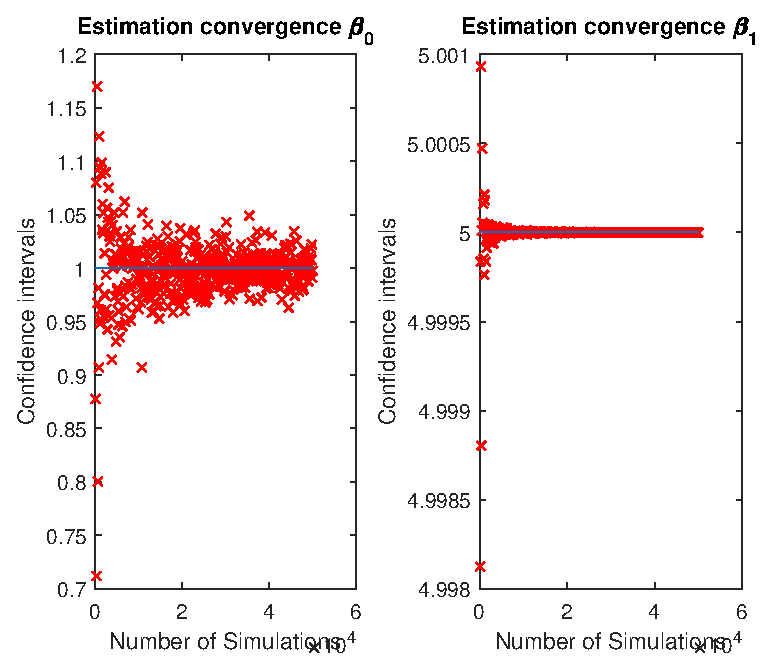
\includegraphics[width=0.55\textwidth]{graphs/fig3.eps}
    \caption{Konvergence odhadů k teoretickým hodnotám v závislosti na rostoucím počtu dat.}
    \label{fig:lr3}
\end{figure}
\FloatBarrier

\section{Závěr}

V semestrální práci jsme ověřili několik statistických vlastností lineární regrese.
Poznatky zjištěné experimentálně odpovídají teorii.
